\documentclass{./cls/hw}
\usepackage{graphicx,mathtools,inputenc,xspace, bm, amssymb,circuitikz}

\title{On-Site Homework 11}
\course{ECEN 2420}
\author{$\boxed{\text{Patrick Harrington}}$}

\begin{document}
\maketitle
\section*{Introduction}
This lab concludes the Norcal 40A assembly and includes the final radio
alignment.
\section{Installation of remaining components}
  The highlighted items in Figure~\ref{fig:f} were installed on the Norcal
  board.
  \begin{figure}[h!]
    \centering
    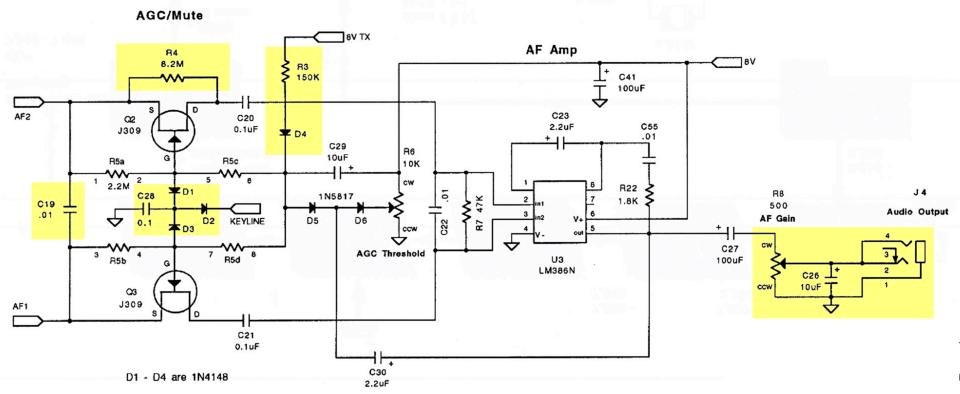
\includegraphics[scale=.5]{./img/final.png}
    \label{fig:f}
    \caption{Remaining parts for the Norcal 40A}
  \end{figure}
  All temporary resistors and wires were removed before the parts were
  installed. 
\section{Initial Settings}
  \begin{enumerate}
    \item All (4) jacks, (2) switches, (3) trimpots, (6) trimcaps, (3) pots had
      their locations noted.
    \item Key jack $J_3$ and the antenna jack $J_1$i were kept disconnected.
    \item A 3.5mm stereo jack was plugged into $J_4$, which is the audio output
      jack.
    \item The trimmer potentiometers were adjusted according to the following specs:
      \begin{itemize}
        \item $R_6$ was set to maximum (clockwise) to disable the AGC.
        \item $R_8$ was set to maximum (clockwise) so that the audio was at the highest
          value.
        \item $R_{13}$ was set completely counter-clockwise so the transmitter
          drive was at the lowest value.
      \end{itemize}
    \item The main potentiometers were then set
      \begin{itemize}
          \item $R_2$ was set fully clockwise so the RF gain was maxed out.
      \end{itemize}
    \item Switch $S_1$ was set off (down position) so the power would be off
    \item Switch $S_2$ was also set in the down position so the RIT would be
      disabled.
  \end{enumerate}
\section{Final Checklist}
Before proceeding to the final calibration leg, the following steps were taken
to ensure everything went along properly.
\begin{enumerate}
  \item DC Power Supply set to 12.0V, current limited to 100mA.
  \item The power cable was attached to the Norcal 40A and $S_1$ was turned on
    (up position). The DC current was measured to be $\boxed{mA}$ which fell in the
    expected range between 15mA and 18mA.
  \item Using a proper CW keyer, the DC current draw was then measured. The
    range of values was between 25mA and 55mA, the measured DC current draw
    with the key active was $\boxed{mA}$.
  \item Ater these measurements were taken, the keyer was detached from the key
    jack $J_3$.
\end{enumerate}

\section{Calibration}
With the pre-calibration steps carefully completed, we proceeded to follow the
following through exactly as directed:
\subsection{External Equipment Setup}
\begin{enumerate}
  \item The signal generator was set to output $4mV_{pp}$ into 50$\Omega$ at a
    frequency of $7.040MHz$.
  \item The signal generator was connected to a 40dB attenuator and was
    attached appropriately to the Norcal 40A.
  \item The Oscilloscope was then calibrated to measure 200$mV$ per division
    and the time base 200$ns$ per division. The channel was set for a X10 probe
    with AC coupling. The scope was then set to measure frequency and Voltage
    in $V_{pp}$.
  \item The scope probe was then connected to the test point wire near switch
    $S_2$ and the scope ground was grounded on a reliable ground.
\end{enumerate}
\subsection{Calibrating the VFO}
\begin{enumerate}
  \item With the scope probe set to 10:1, the signal was measured to be within
    600 and 800 $mV_{pp}$ at $\boxed{mV_{pp}}$
  \item With $R_{17}$ set at half position, $C_{50}$ was adjusted until the VFO frequency was at 2.
    125MHz.
  \item $R_{17}$ was then set counterclockwise and the frequency was measured
    to be $\boxed{ MHz\pm 100Hz}$
  \item $R_{17}$ was then set fully clockwise and the frequency was measured
    to be $\boxed{ MHz\pm 100Hz}$
  \item $R_17$ was then adjusted until the frequency was as close to possible
    to 2.125MHz.
  \item The freq range of the radio was found to be approximately $\boxed{
    Hz\pm 200Hz}$
\end{enumerate}
\subsection{Receiver Alignment}
\begin{enumerate}
  \item The scope was again checked so that it measured 200mV per division,
    and the time base was set to 2ms per division.
  \item $C_{17}$ was adjusted so that the measured frequency was 575$\pm 10Hz$
  \item The measured audio voltage was found to be $\boxed{ mV_{pp}}$
  \item The RF signal generator was adjusted such that a 6dB ($\approx$4x) change was observed.
  \item The 6dB bandwidth was measured to be $\boxed{ Hz}$
  \item The RF signal was then adjusted until it was near 575$Hz$.
  \item Next, the RIT was set on by turning on $S_2$, and $R_16$ was adjusted
    and the frequencies were noted. The range of frequencies was found to be
    $\boxed{ Hz}$
  \item The RIT switch $S_2$ was turned off and the audio frequency was
    returned to $\approx$ 575$Hz$.
  \item The AGC potentiometer $R_6$ was adjusted such that the voltage at the
    scope dropped by $\frac{1}{3}$.
  \item Finally, the function generator was disconnected from the 30dB
    attenuator with the pad still connected to $J_1$.
\end{enumerate}
\subsection{Transmitter Alignment}
\begin{enumerate}
  \item The scope was set to read 50mV per division and the time base set to 2ms
    per division.
  \item The DC supply was set with a limit at 200mA
  \item $R_{13}$ was set to be at half-value.
  \item The CW keyer was connected $J_3$
  \item $C_{39}$ (TX filter) was set to yield max voltage at an audio frequency
    on the scope, where the trimcap $C_{39}$ was not near either extreme value.
  \item The DC current draw was measured to be $\boxed{ mA}$
  \item $C_{34}$ (TX frequency) was adjusted to be $\approx575Hz\pm10Hz$
  \item The scope was then set to read 2V per division and the time base was
    set to 200ns per division. The scope was attached to the TX end of the 30dB
    attenuator (which was not the open end).
  \item The 40dB attenuator was found to reduce the power by a factor of
    $\boxed{ }$
  \item The RF voltage was measured in order to calculate the transmitter
    power, which was found to be $\boxed{ W}$
  \item The short on $J_3$ was removed.
  \item The DC power supply was limited to 600mA
  \item The scope was set to read 5V per division
  \item $R_{13}$ was set to full clockwise position, and the RF voltage was
  measured, taking care to keep the transmitter from running for more than a
  few seconds at max power. The full-power voltage was found to be $\boxed{ V}$.
\item $R_{13}$ was then set to 50\% value, the RF voltage was found to be
  $\boxed{ V}$.
  \item The maximum power the transmitter can provide was found to be $\boxed{
    W}$
\end{enumerate}
\end{document}
